\documentclass[../main.tex]{subfiles}
\begin{document}
	

	\chapter{Theorem and proof} \label{ch:proof}
\noindent  The work revolves around the following theorem and its proof. 
	\section{Theorem}
	\begin{theorem} Let $ \sigma \in  \mathcal{M}$. Set
		$$ \Sigma_n = span\{\sigma(w\cdot x + \theta) : w\in \mathbb{R}^n, \theta \in \mathbb{R} \}.$$
		Then $\Sigma_n$ is dense in $\mathcal{C}(\mathbb{R}^n)$ if and only if $\sigma$ is not a polynomial. 
	\label{teorema}
	\end{theorem}


\subsection{Previous results}
\noindent  There has been significant research on the approximation capabilities of feedforward networks prior to the proof of this theorem. Previous studies have demonstrated that if the activation functions of the network satisfy certain explicit assumptions, then the network can be proven to be as they call it, a universal approximator. For instance, \cite{HORNIK1991251} have established two results, which are as follows:

\begin{theorem} (Hornik Theorem 1). Multilayer feedforward networks with a bounded and nonconstant activation function can approximate any function in $L^p(\mu)$ arbitrary well, given a sufficiently large number of hidden units. 
\end{theorem}

\begin{theorem} (Hornik Theorem 2) Multilayer feedforward networks with a continuous, bounded and nonconstant activation function can approximate any continuous function on $X$ arbitrarily well (with respect to the uniform distance) given a sufficiently large number of hidden units. 
\end{theorem}

\noindent
The Theorem \ref{teorema} generalizes Hornik's Theorem 2 by establishing necessary and sufficient conditions for universal approximation. Note that the theorem merely requires "nonpolynomiality" in the activation function. Unlike Hornik's result, the activation functions do not need to be continuous or smooth. This has an important biological interpretation because the activation functions of real neurons may well be discontinuous or even non-elementary.

	\section{Proof}
	\subsection{If $\sigma$ is not a polynomial then $\Sigma_n$ is dense in $\mathcal{C}(\mathbb{R}^n)$ }
	\noindent Consider that $\sigma$ is not an algebraic polynomial and we aim to show that $\Sigma_n$ is dense in $\mathcal{C}(\mathbb{R}^n)$. In order to show that, we devided the proof in 3 steps, each one aims to proof one proposition that needs some previous Lemmas. 
	
	\subsubsection{Step 1}
	\begin{propo} \label{prop1}
		If $\sigma$ is not a polinomial then $\sigma \ast \varphi$ is not a polynomial for some $\varphi \in \mathcal{C}^\infty_0$.  
	\end{propo}
	\noindent To proof this proposition we need the following two lemmas. 
	\begin{lema}  \label{lemma1}
		If we have that $\sigma \ast \varphi $ is a polynomial for all $\varphi \in \mathcal{C}^\infty_0 $, then the degree of the polynomial $\sigma \ast \varphi $ is finite, i.e. there exists an $m$ $\in \mathbb{N}$ such that $ deg (\sigma \ast \varphi) \leq m$ for all $\varphi \in \mathcal{C}^\infty_0$. 
	\end{lema}
	\begin{proof}
		We first prove the claim in the case of $\varphi \in \mathcal{C}^\infty_0[a,b]$, for some $a<b$. \\ \\ By Proposition \ref{prop:frech} we have that $(\mathcal{C}^\infty_0[a,b],\rho)$ is a complete metric space.  \\ \\  Consider the following set, \\ $$V_k= \{\varphi \in \mathcal{C}_0^\infty[a,b] \, | \,  deg(\sigma \ast \varphi ) \leq k\}.$$ \\
		It is clear that this set $V_k\subseteq \mathcal{C}_0^\infty[a,b]. $ 
		We want to show that $\mathcal{C}_0^\infty[a,b] = V_k.$ \\ \\  The set $ V_k$ fulfills the following properties: $V_k \subset V_{k+1}$, $V_k $ is a closed subspace, $\cup_{k=0}^\infty V_k = \mathcal{C}_0^\infty[a,b]$ and $V_k$ is a vector space. We can easily see that $\mathcal{C}_0^\infty[a,b]$ is also a vector space.\\ \\ 
	\noindent As $\mathcal{C}_0^\infty[a,b]$ is a complete metric space, by Baire's Category Theorem \ref{baire}, this set is of category $II$, i.e. $\mathcal{C}_0^\infty[a,b]$  cannot be written as a countable union of nowhere-dense sets. Recall that $\mathcal{C}_0^\infty[a,b]$ can be written as a countable union of $V_k$, therefore some $V_m $ is not a nowhere-dense set, that is, there exists an open set $U\subseteq C_0^\infty[a,b]$ that is contained in the closure of $V_m$, but, as $V_m$ is closed, for that we have that $U\subseteq V_m$. For topology results, any open set of a vector space contains a basis of the vector space, in our case $U$ contains a baisis of $\mathcal{C}_0^\infty[a,b]$ , and $U\subseteq V_m$, therefore $V_m$ contains a baisis of $\mathcal{C}_0^\infty[a,b]$. Now we can conclude that $\mathcal{C}_0^\infty[a,b] \subseteq V_k.$ And consequently $\mathcal{C}_0^\infty[a,b] = V_k.$ This means that any $\varphi \in \mathcal{C}^\infty_0[a,b] $ also satisfies $ \varphi \in V_k$,  that means that the convolution $\sigma \ast \varphi $ has degree finite. \\ 
		
		\noindent For the general case where $\varphi \in \mathcal{C}_0^\infty$, we note that the number $m$ does not depend on the interval $[a,b]$. This can be seen as follows. By translation $m$ depends at most of the length of the interval. Let $[A,B]$ be any interval. For $\varphi \in \mathcal{C}^\infty_0[A,B]$ we can find $\varphi_i \in \mathcal{C}^\infty_0[a_i,b_i]$ for $i=1,...,k$ such that $[A,B] \subset \cup_{i=1}^k[a_i,b_i]$ where $b_i -a_i =b-a$ and $\varphi=\sum_{i=1}^k \varphi_i$ Thus $$\sigma \ast \varphi = \sum_{i=1}^k \sigma \ast \varphi_i$$ and for every $i=1,...,k $ we have that $\sigma \ast \varphi$ is a polynomial of degree less than or equal to m. Therefore $deg(\sigma \ast \varphi) \leq m$.
	\end{proof}
	\begin{lema}  \label{lemma2}
		If $\sigma \ast \varphi$ is a polynomial such that $ deg (\sigma \ast \varphi) \leq m$ for all $\varphi \in \mathcal{C}^\infty_0$, then $\sigma$ is a polynomial of degree at most $m$. 
	\end{lema}
	\begin{proof} 
	If $\sigma \ast \varphi$ is a polynomial of degree $m$.
	For all $\varphi \in \mathcal{C}^\infty_0$, using (\ref{prop:2}) we have that
	$$(\sigma \ast \varphi)^{(m+1)} \, (x)=\int \sigma(x-y)\varphi^{(m+1)}(y) \, dy= 0$$  
	From standard results in Distribution Theory [pp 57 \cite{friedman1963generalized}], $\sigma $ is itself a polynomial of degree at most $m$ (a.e.).
	\end{proof} 
\vspace{\baselineskip} 

\begin{proof}[Proof of Proposition \ref{prop1}]
We will show the contrapositive. Suppose that the convolution $\sigma \ast \varphi$ is a polynomial for all $\varphi \in \mathcal{C}^\infty_0$, by Lemma \ref{lemma1} the degree of the convolution is finite. Now we have that $\sigma \ast \varphi$ is a polynomial of finite degree, by Lemma \ref{lemma2} we have that $\sigma$ is a polynomial. 
\end{proof}
\vspace{\baselineskip} 
\subsubsection{Step 2}

	\begin{propo}  \label{prop2}
	If for some $\varphi \in \mathcal{C}^\infty_0 $ we have that $\sigma \ast \varphi $ is not a polynomial, then $\Sigma_1$ is dense in $\mathcal{C}(\mathbb{R})$.
\end{propo}

	\begin{lema}  \label{lemma3}
		For each $\varphi \in  \mathcal{C}^\infty_0$, $ \sigma \ast \varphi \in  \overline{\Sigma_1}$. 
		
	\end{lema}
	
	\begin{proof} % proof step 4
		We recall the definition of the set 
		\begin{equation}
			\Sigma_1 = \text{span} \{ {\sigma(w\cdot x + \theta) : w\in \mathbb{R}, \theta \in \mathbb{R} \} }.
			\tag{1}
			%\label{eq:ecuacion1}
		\end{equation}
	Without loss of generality, assume that $\text{supp }\varphi \subseteq [-\alpha,\alpha] $.
	To show that $\sigma \ast \varphi \in \overline{\Sigma_1} $ we will use the characterization for elements in the closure. We will to prove that there exists a sequence in $\Sigma_1$ such that uniformly converges to $\sigma \ast \varphi$ on $[-\alpha,\alpha]$. Note that we usually denote for un$\rightrightarrows$) \\ 
	
	\noindent We shall consider the following sequence: 
		$$h_m= \sum_{i=1}^m\varphi(y_i)\Delta y_i \sigma(x-y_i).$$ 
		Which satisfies $h_j\in \Sigma_1$ for $j=1,...,m$. Note that we have $w_i=1,\theta_i=-y_i$ and $  \beta_i=\varphi(y_i)\Delta y_i$.\\ \\ 
		
		\noindent We will define a partition of the interval $[-\alpha,\alpha]$ to be the following, where $$y_i=-\alpha + \frac{2i\alpha}{m}\quad i=1,...,m$$ and $\Delta y_i=\frac{2\alpha}{m}$. \\ \\
		Given $\epsilon >0$, we choose $\delta >0$ such that $$10\delta \| \sigma\|_{L^\infty\{-2\alpha,2\alpha\}}\|\varphi \|_{L^\infty} \leq \frac{\epsilon}{3}.$$
		We know that $\sigma \in M$. Hence, for the previous choosen $\delta>0$ and $[-\alpha,\alpha]$ interval, there exists $r(\delta)$ finite number of intervals the measure of whose union $U$ is $\delta$ such that $\sigma$ is uniformly continuous on $[-2\alpha,2\alpha]/U$. We now choose $m_i$ sufficiently large so that
		\begin{enumerate}
			\item $m_1 \delta > \alpha r(\delta)$. We can do this by Archimedes' principle.
			\item From the uniform continuity of $\varphi$ we know that \\
			
			if $|s-t| \leq \delta_2= \frac{2 \alpha }{m_2}$ then $$|\varphi(s)- \varphi(t)| \leq \epsilon_2= \frac{\epsilon}{2 \alpha \| \sigma\|_{L^\infty[-2\alpha,2\alpha]}}$$
			\item From the previous, $\sigma$ is uniformly continuous on  $[-2\alpha,2\alpha]/ U$ thus we have,\\ 
			 
			 if $s,t \in [-2\alpha, 2\alpha]/U$ and $|s-t|\leq \delta_3 = \frac{2\alpha}{m_3}$ then $$|\sigma(s)-\sigma(t)| \leq \epsilon_3= \frac{\epsilon}{\|\varphi\|_L}$$
		\end{enumerate}
		We choose $m$ such that $m=max\{m_1,m_2,m_3\}$. \\ \\ 
		Now, fix $x\in [-\alpha,\alpha] $. Set $\Delta_i= [y_{i-1},y_i]$ where $y_0= \alpha$. \\ \\
		First, recall that,\\
		$$\int \sigma(x-y)\varphi(y)dy = \sum_{i=1}^m \int_{\Delta_i}\sigma(x-y)\varphi(y)dy.$$
		\\ Consider the following difference:

\begin{equation*} 
	\begin{split}
		\Bigg| \int \sigma(x-y)\varphi(y)dy -  \sum_{i=1}^m \int_{\Delta_i}& \sigma(x-y_i) \varphi(y)dy \Bigg|  \\
		& = \left|  \sum_{i=1}^m \int_{\Delta_i}\sigma(x-y)\varphi(y)dy -  \sum_{i=1}^m \int_{\Delta_i}\sigma(x-y_i)\varphi(y)dy \right|  \\
		& =  \left|  \sum_{i=1}^m \int_{\Delta_i}\varphi(y)\Big( \sigma(x-y) - \sigma(x-y_i)\Big)dy \right| \\
		&\leq  \sum_{i=1}^m \int_{\Delta_i} \left| \varphi(y)\right| \left| \sigma(x-y)-\sigma(x-y_i)\right|dy.
	\end{split}
\end{equation*}
		If $x-\Delta_i \cap U = \varnothing $. Since $x-y \notin U$ , $x-y_i \notin U$ and $x-y_i \in [-2\alpha,2\alpha]$. For choice of $m$ in property 2, we have
		
		\begin{multline*}
			\sum_{i=1}^m  \int_{\Delta_i} \left| \varphi(y)\right| \left| \sigma(x-y)-\sigma(x-y_i)\right|dy  \leq  \frac{\epsilon}{\| \varphi\|_{L_1}}  \sum_{i=1}^m  \int_{\Delta_i} \left| \varphi(y)\right| \\ =  \frac{\epsilon}{3\| \varphi\|_{L_1}} \int \left|\varphi(y)\right| dy =  \frac{\epsilon}{3\| \varphi\|_{L_1}} \left|\varphi(y)\right|_{L_1}  = \frac{\epsilon}{3} . 
		\end{multline*}
	\\ 
		\noindent If $x-\Delta_i \cap U \neq \varnothing$ then we will denote such intervals by $\tilde{\Delta_i}.$\\ \\ 
		$\sum_i |\tilde{\Delta_i}| = \sum_i|(x-\Delta_i \cap U)| \leq |U|+2|\Delta_i| r(\delta) \leq \delta + 2 \cdot \frac{2\alpha}{m} r(\delta) \leq \delta +4\delta = 5\delta$  \\ \\ 
		We used the property $m\delta > \alpha r(\delta) $,  indeed $ \delta > \frac{\alpha \cdot r(\delta)}{m}$. 
		
		
		\begin{multline*}
			\begin{split}
				\sum_{i=1}^m  \int_{\tilde{\Delta_i}} \left| \varphi(y)\right| \left| \sigma(x-y)-\sigma(x-y_i)\right|dy  \leq  \sum_{i=1}^m  \int_{\tilde{\Delta_i}} \| \varphi\|_{L^{\infty}} \, 2 \| \sigma \|_{L^{\infty}[-2\alpha,2\alpha]} \\
				 = \| \varphi\|_{L^{\infty}} \, 2 \| \sigma \|_{L^{\infty}[-2\alpha,2\alpha]} \sum_i| \tilde{\Delta_i} | \\
				 \leq \| \varphi\|_{L^{\infty}} \, 2 \| \sigma \|_{L^{\infty}[-2\alpha,2\alpha]} \, 5 \delta \leq \frac{\epsilon}{3}
			\end{split}
		\end{multline*}
		Moreover, 
\begin{equation*} 
	\begin{split}
		\Bigg| \sum_{i=1}^m \int_{\Delta_i} \sigma(x-y_i)\varphi(y)dy -  \sum_{i=1}^m &\sigma(x-y_i) \varphi(y_i)\Delta y_i \Bigg| \\
		& =  \left|  \sum_{i=1}^m \int_{\Delta_i} \sigma(x-y_i) [\varphi(y)-\varphi(y_i)] dy \right| \\
		& \leq  \sum_{i=1}^m \int_{\Delta_i}  \left| \sigma(x-y_i)\right| \left| \varphi(y) - \varphi(y_i)\right|dy  \\
		& \leq  \sum_{i=1}^m \int_{\Delta_i}  \left| \sigma(x-y_i)\right| dy \left[ \frac{\epsilon/3}{2\alpha \| \sigma\|_{L^\infty[-2\alpha,2\alpha]}}\right]  \leq \frac{\epsilon}{3} 
	\end{split}
\end{equation*}
Finally, we have the result $h_m \rightrightarrows \sigma \ast \varphi $ because

$$\Bigg| \int \sigma(x-y)\varphi(y)dy -  \sum_{i=1}^m \sigma(x-y_i) \varphi(y_i) \Delta y_i \Bigg| \leq \epsilon $$
\\ for all $x\in [-\alpha,\alpha ].$
	\end{proof}
	\vspace{\baselineskip} 
	%\subsubsection{$\Sigma_1$ dense in $\mathcal{C}(\mathbb{R})$}
	\begin{lema}  \label{lemma4}
		If $\sigma \in \mathcal{C}^{\infty}$, then $ \Sigma_1$ is dense in  $\mathcal{C}(\mathbb{R})$.
	\end{lema}
	
	\begin{proof} % proof step 3
		We suppose that  $\sigma \in \mathcal{C}^{\infty}$ and recall by the theorem hypothesis $\sigma$ is not a polynomial. 
		 We can write any function $f$ of the set $\Sigma_1$ as $$f=\sum_i \beta_i \sigma_i(w_i x+\theta_i)= \beta_1 \sigma_1(w_1 x+\theta_1)+ ... $$ 
		We can see that the function $$\frac{\sigma([w+h]x + \theta) - \sigma(wx+\theta)}{h} \in \Sigma_1$$ because is a linear combination, where $\beta_1= \frac{1}{h}, \beta_2=\frac{-1}{h}$. \\ \\  By hypothesis, $\sigma \in \mathcal{C}^{\infty}$. By definition of derivative we have
		$$ \frac{d}{dw}\sigma(wx+\theta)= \lim_{h \to 0} \frac{\sigma([w+h]x + \theta) - \sigma(wx+\theta)}{h}  \in \overline{\Sigma_1} %\footnote{$\overline{\Sigma_1}$ denotes the clausure of the set $\Sigma_1$}
		$$
		because the limit of a set belongs to the closure of the set. \\  \\ 
		By the same argument, $$\frac{d^k}{dw^k} \sigma(wx+\theta) \in \overline{\Sigma_1}$$  for all $k\in \mathbb{N}, w,\theta \in \mathbb{R}$.\\ \\ 
		 If we differentiate this expression k times, we obtain 
		$$ \frac{d^k}{dw^k}\sigma(wx+\theta) = \sigma^{(k)}(wx+\theta) \cdot x^{k}$$
		We are going to see that if $\sigma$ is not a polynomial (by hypothesis) then there exists a $\theta_k\in \mathbb{R}$ such that $\sigma^{(k)}(\theta_k)  \neq 0$. To show that, let us assume that does not exist any $ \theta_k \in \mathbb{R}$ such that $\sigma^{(k)}(\theta_k)  \neq 0$. This means that the k-th derivative at every point is 0, i.e. $$\sigma^{(k)}(\theta)=0  \quad \forall \theta \in \mathbb{R} $$
		\noindent  If we integrate this expression, we will have
			$\int \sigma^{(k)}= \int 0$. This implies that $$\sigma^{(k-1)}(x) = C_1$$ for some constant $C_1$, as integrating zero results in a constant. If we integrate again, we have: $$\sigma^{(k-2)}(x) = C_1x + C_2$$ for some constants $C_1$ and $C_2$.
		
		\noindent Continuing this process, we arrive at $$\sigma(x) = C_1x^{k-1} + C_2x^{k-2} + \ldots + C_{k-1}x + C_k$$ for constants $C_1, C_2, \ldots, C_k$. Hence, $\sigma$ is a polynomial of degree $k-1$, which contradicts our assumption that $\sigma$ is not a polynomial. Therefore, there always exists a point where the derivative does not vanish. \\  \\ 
		Thus, we evaluate at the point where the derivative does not vanish, we call it $\theta_k$.
		$$  \sigma^{(k)}(\theta_k) \cdot x^{k}=\frac{d^k}{dw^k}\sigma(wx+\theta) \Bigr|_{w=0, \theta=\theta_k} \in  \overline{\Sigma_1} $$ 
		This implies that $\overline{\Sigma_1}$ contains all polynomials, because the expression $\sigma^{(k)}(\theta_k) x^{k}$ generates all polynomials. By the Weierstrass theorem, we know that the polynomials are dense in $\mathcal{C}(\mathbb{R})$. This concludes that the set $\overline{\Sigma_1}$ contains a set which is dense in  $\mathcal{C}(\mathbb{R})$, therefore $\Sigma_1$ is dense in $\mathcal{C}(\mathbb{R})$.
	\end{proof} 
\vspace{\baselineskip} 
	 \begin{proof}[Proof of Proposition \ref{prop2}]
	 From Lemma \ref{lemma3}, $\sigma \ast \varphi \in  \overline{\Sigma_1}$ for each $\varphi \in \mathcal{C}^\infty_0$. It immedialy follows that, $\sigma \ast \varphi (wx+\theta ) \in  \overline{\Sigma_1}$, for each $ w, \theta \in \mathbb{R}$ and $\varphi \in \mathcal{C}^\infty_0$.\\ 
	 Now, we shall see the results in distributions \ref{prop:29} to proof the following result. For $\sigma$ and $\varphi \in \mathcal{C}^\infty_0$, we have that $\sigma \ast \varphi \in  \mathcal{C}^\infty $.
	 From Lemma \ref{lemma4} applied in $\sigma= \sigma \ast \varphi$, if $\sigma \ast \varphi \in  \mathcal{C}^\infty $, then $\Sigma_1$ dense in $\mathcal{C} (\mathbb{R})$. 
	 \end{proof}
\vspace{\baselineskip} 
\subsubsection{Step 3}
\noindent We will prove that approximating a $\mathcal{C}(\mathbb{R})$ function  with one from the set $\Sigma_1$ implies approximating a function $\mathcal{C}(\mathbb{R}^n)$ from the set $\Sigma_n$. We can see this from the density characterization.

	\begin{propo}  % L6: step 2
			If $\Sigma_1$ is dense in $\mathcal{C}(\mathbb{R})$, then $\Sigma_n$ is dense in $\mathcal{C}(\mathbb{R}^n)$. 
		\end{propo}
	
	\begin{proof} % proof  step 2
			The following proof is inspired by \cite{chui_approximation}.\\ \\ Consider the set $$V:= span\{ f(ax) : a \in \mathbb{R}^n, f \in \mathcal{C}(\mathbb{R}) \}.$$ First, we shall see that $V$ is dense in $\mathcal{C}(\mathbb{R}^n)$.  If we show that $V$ contains the polynomials, which are dense in $C(\mathbb{R}^n)$ by Weierstrass Theorem, that will be enough. \\ \\
			\noindent In fact, we have the set $$ H = \langle (a x)^k\rangle = span\{ p(ax) : a \in \mathbb{R}^n, \, p \in \mathbb{R}[x] \} \subseteq V.$$ \\
			We only need to show that $H:=\mathbb{R}[x]$, in other words, that the polynomials of degree $k$ can be generated by $(a\cdot x)^k$. For the isomorphism theorem, we know that
			
			 $$\mathbb{R}[x]^*/\text{ann(H)}\cong H^*$$
			 \\ 
			 Since $$D^{m_1} x^{m_2}= \delta_{m_1,m_2}k!, $$ we see that $\mathbb{R}[x]^*$ can be generated by $\langle D^{m_1}\rangle _{|m_1|=k}$. Consider any element of $\mathbb{R}[x]^*$, say $\sum \alpha_j D^{m_j}$ and suppose that annihilates  $H$. That is $$(\sum \alpha_j D^{m_j} ) x^{m_j}=\alpha_j k! = 0.$$ \noindent This implies that $\text{for all } j,\, \alpha_j =0$ and then the element $\sum \alpha_j D^{m_j}=0$
			 For that reason, it means that $ann(H)=0$ which implies that $\mathbb{R}[x]^*\cong H^*$, which is what we wanted to see. Thus, we have the set $V$ dense in $\mathcal{C}(\mathbb{R})$.
			\\ \\ 
			\noindent Let $g\in \mathcal{C}(\mathbb{R}^n) $, for any compact subset $K \subset \mathbb{R}^n  $, $V$ dense in $\mathcal{C}(K)$. That is, given $\epsilon >0$, there exist $f_i\in  \mathcal{C}(\mathbb{R})$ and $a_i \in \mathbb{R}^n $    {\scriptsize $i=1,...,k$}  such that
			
			$$ \big| g(x)-\sum_{i=1}^k f_i(a^i \cdot x) \big| < \frac{\epsilon}{2}$$
			for all $x\in K$. We now consider the set of all the points in the compact $K$ multiplied by the vector $a^i$. That is $\{a^i \cdot x | x \in K\}$ $\subseteq[\alpha_i,\beta_i] $ for some finite interval $[\alpha_i,\beta_i]$, $i=1,...,k$. By hypothesis $\Sigma_1 $ dense in $\mathcal{C}(\mathbb{R})$, specifically $\Sigma_1 $ is dense in $[\alpha_i,\beta_i ]$ $ \, i=1,...,k$. Hence there exist constants $c_{ij}, w_{ij}$ and $\theta_{ij}$, $j=1,...,m_i$, $i=1,...,k$ such that 
			
			$$ \big|f_i(y) - \sum_{j=1}^{m} c_{ij} \sigma(w_{ij}y+ \theta_{ij})\big| < \frac{\epsilon}{2k}$$
			for all $y\in [\alpha_i,\beta_i ]$. \\ \\
			Therefore, 
			$$ \big| g(x) - \sum_{i=1}^k \sum_{j=1}^m c_{ij} \sigma(w_{ij}(a^i \cdot x) + \theta_{ij})  \big| < \epsilon$$
			for all $x\in K$. We have shown that  $\Sigma_n$ is dense in $\mathcal{C}(\mathbb{R}^n)$ which is what we wanted.
		\end{proof}


\section{Proof of Theorem \ref{teorema}}
	\begin{proof}~ % proof del teorema

	\begin{enumerate}
		\item[$\Rightarrow$] 
		To prove this implication statement, we aim to show that if $\Sigma_n$ is dense in $\mathcal{C}(\mathbb{R}^n)$, then $\sigma$ is not a polynomial.
		 We will proceed to prove the contrapositive statement, assuming that $\sigma$ is indeed a polynomial, and demonstrate that in this case, $\Sigma_n$ cannot be dense in $\mathcal{C}(\mathbb{R}^n)$. \\ \\ Let $\sigma$ be a polynomial of degree k, then $\sigma(wx+\theta)$ is a polynomial  of degree k for every $w,\theta$. Recall that $$ \Sigma_n = span\{\sigma(w\cdot x + \theta) : w\in \mathbb{R}^n, \theta \in \mathbb{R} \}$$  that is the set of algebraic polynomials of degree at most k. To show that $\Sigma_n$ is not dens in $\mathcal{C}(\mathbb{R}^n)$, for the definition of density, we need to find a function $f(x)\in \mathcal{C}(\mathbb{R}^n)$, $\epsilon > 0$ and $K$ such that  $\| p-f \| > \epsilon$ for all $p$ polynomial of degree k. For example, let $f(x)=cos(x)$, and let $p(x)= \sigma(wx+\theta)$ that has degree at most k. This implies has maximum k roots. We can find a interval where $cos(x)$ has k+1 roots. Therefore, $\Sigma_n$ is not dense in $\mathcal{C}(\mathbb{R}^n)$. 

		\item[$\Leftarrow$]  In order to prove this implication, we need to show that if $\sigma$ is not an algebraic polynomial, then $\Sigma_n$ is dense in $\mathcal{C}(\mathbb{R}^n)$.
		
		
		 By hypothesis, $\sigma$ is not a polynomial, by Proposition 1 this implies that $\sigma \ast \varphi$ is not a polynomial for some $\varphi \in \mathcal{C}_0^\infty$. By Proposition 2 if $\sigma \ast \varphi$ is not a polynomial for some $\varphi$, then $\Sigma_1$ is dense in $\mathcal{C}(\mathbb{R})$. Finally in Proposition 3 we have showed that this implied that $\Sigma_n$ is dense in $\mathcal{C}(\mathbb{R}^n).$
		 
	\end{enumerate}
\end{proof}


\section{About the theorem}

\subsection{Why does it not contradict the Weierstrass approximation theorem? }

\noindent In mathematical analysis, we prove the Weierstrass approximation theorem, which we will now recall. 
\begin{theorem}(Weierstrass  approximation theorem)
	Let $f:[a,b]\rightarrow \mathbb{R} $ be a continuous function. Then, there exists polynomials $p_n\in \mathcal{R}[x]$ such that the sequence $(p_n)$ converge uniformly to $f$ on $[a,b]$. 
\end{theorem} 

\begin{corolari}
	The set of polynomial functions $\mathcal{R}^n[x]$ is dense in the space of continuous functions on a compact set $K \subset \mathbb{R}^n$, $\mathcal{C}(K)$. So any continuous function on a compact set can be approximated arbitrarly well by a polynomial. 
\end{corolari}

\noindent The theorem \ref{teorema} states that: if $\Sigma_n$ is dense in $\mathcal{C}(\mathbb{R}^n)$ then $\sigma$ is not an algebraic polynomial. But why this statment does not contradict the Weierstrass approximation theorem?
This does not work because $\sigma$ has degree fixed $k$, then any element in the set $\Sigma_n$ has degree at most $k$. Hence, the set $\Sigma_n$ is a finite vector space and can not be dense in $\mathcal{C}(\mathbb{R}^n)$. Not all contiunous functions can be approximated with a polynimial of degree fixed. We argued this in the proof where with the example of the $cosine$ function. For example, if $k=3$, we cannot approximate the cosine function with linear combinations of polynomials of maximum degree 3.

\begin{figure}[h]
	\centering
	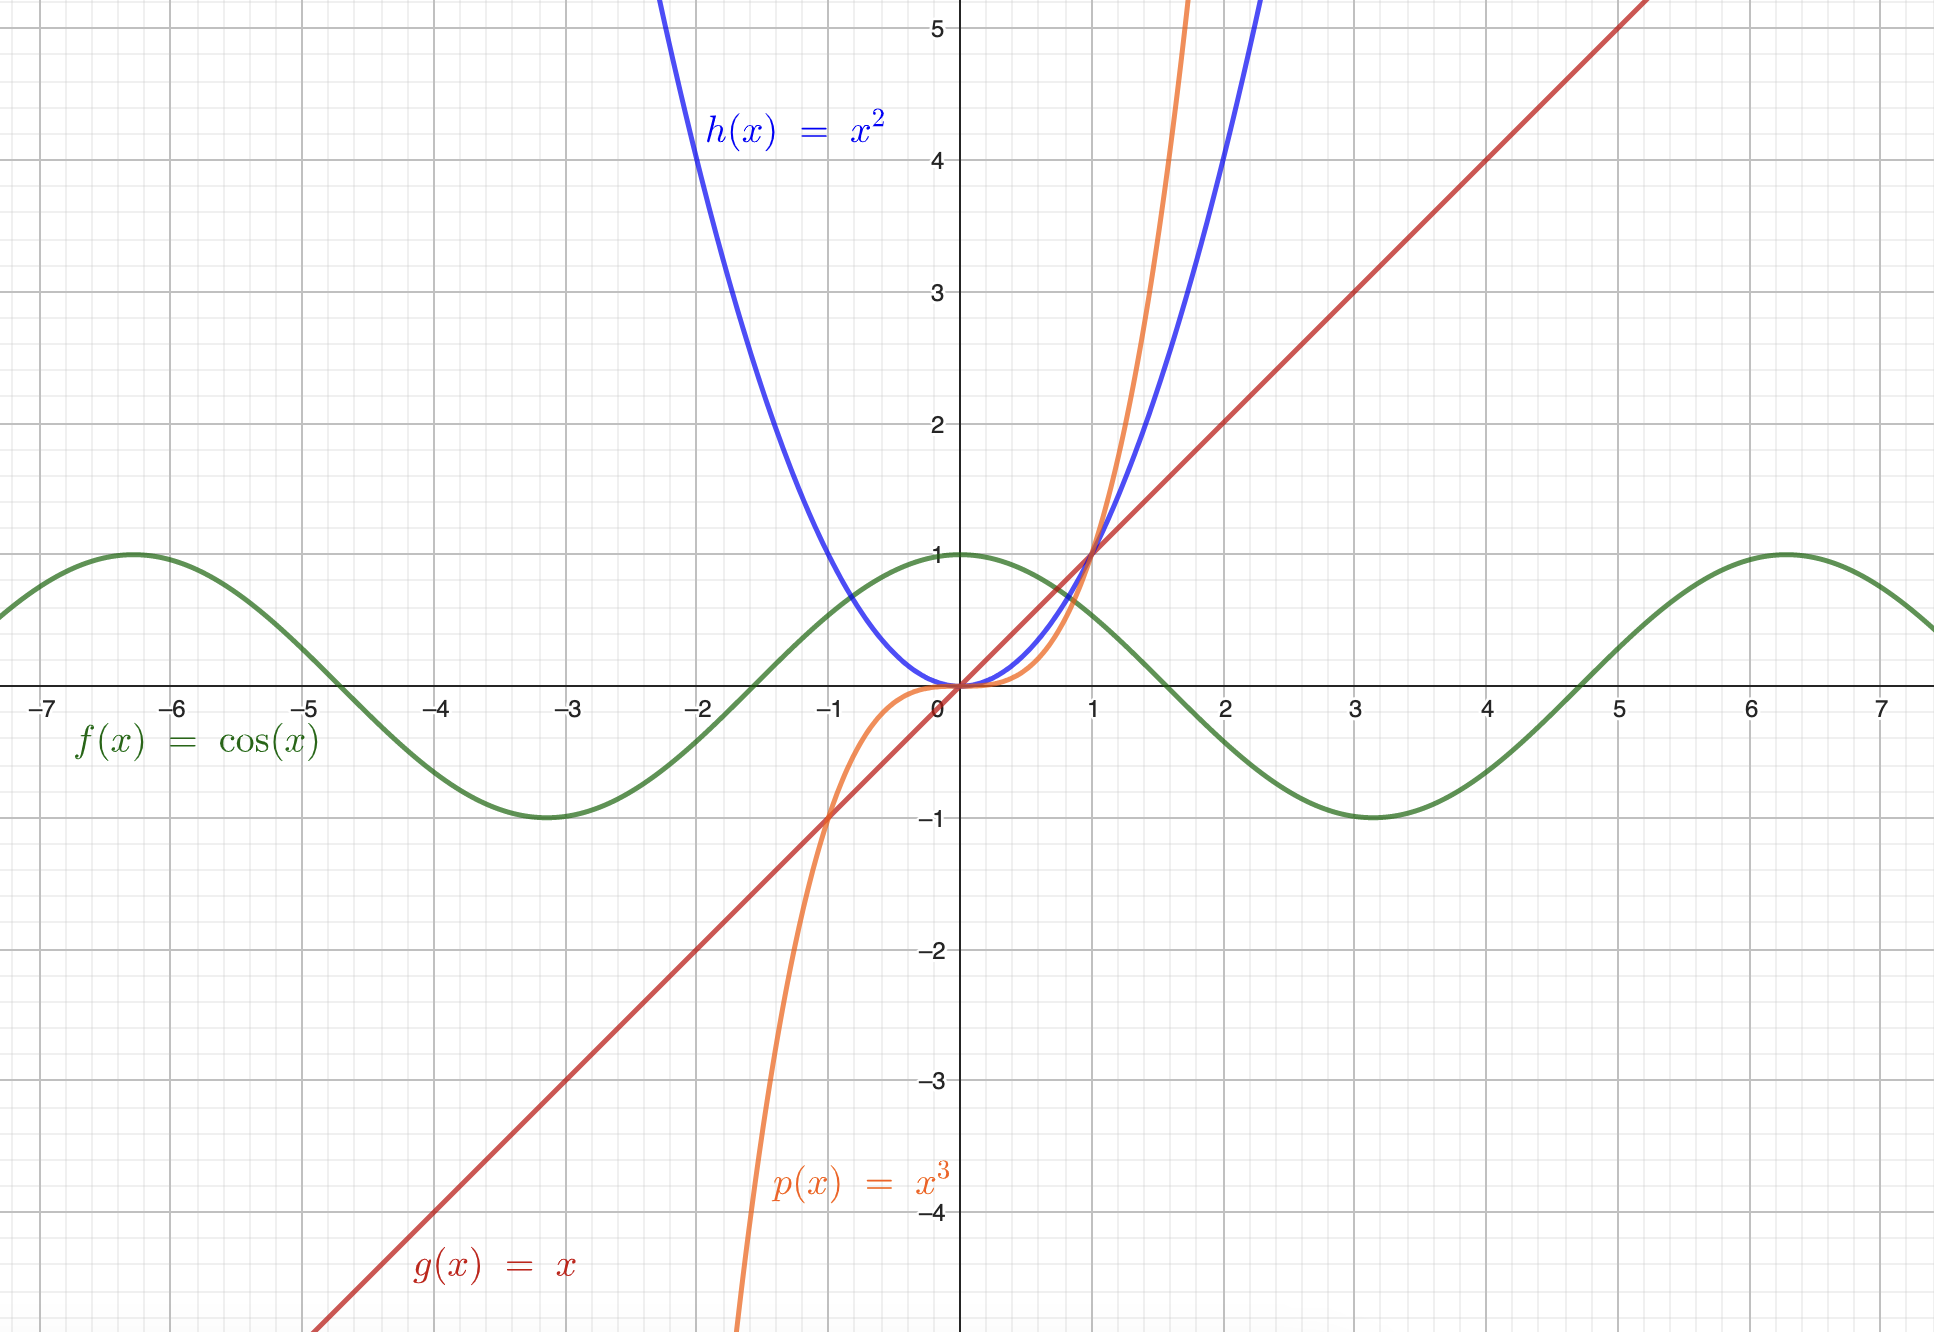
\includegraphics[width=0.6\linewidth]{imgs/cos.png}
	\caption{\small Cosine function cannot be approximated with linear combinations of polynomials of maximum degree 3.} 
\end{figure} \mbox{} \par

\subsection{Conclusion}


	\noindent The theorem only requires the activation function to be non-polynomial; we do not need continuity in sigma. Our finding that the activation function need not be continuous or smooth also has an important biological interpretation because the activation functions of real neurons may well be discontinuous or even non-elementary. Note that the ReLU function mentioned before is commonly regarded as one of the best activation functions in deep learning. We can see that it is non-smooth, and due to the proven theorem, we can still assure that it can be used in any case (because it is non-polynomial).
\subsection{Corollaries}


\begin{definition} The set $L^{p}(\mu)$ contains all mesurable functions $f$ such that: 
	$$ \|f\|_{L^p}(\mu) = \Big( \int_{R^n} |f(x)|^p d\mu(x)\Big)^{1/p} < \infty. $$
	
\end{definition}

\begin{propo}
	Let $\mu $ be a non-negative finite measure on $\mathbb{R}$ with compact support, absolutely continous with respect to Lebesgue measure. Then $\Sigma_n$ is dense in $L_p(\mu)$ , $1\leq p < \infty$, if and only of, $\sigma$ is not a polynomial.
\end{propo}

\begin{propo}
	If $\sigma\in M$ is not a polynomial (a.e) then, $$ \Sigma_n(\mathcal{A})= span \{ \sigma(\lambda w \cdot x + \theta) : \lambda, \theta \in \mathbb{R}, w \in \mathcal{A} \}$$
	is dense in $\mathcal{C}(\mathbb{R}^n)$ for some $\mathcal{A}\subset \mathbb{R}^n$ if and only if there does not exist a nontrivival polynomial vanishing on $\mathcal{A}$.
\end{propo}
 
\end{document}